% StickForStats: A Statistical Analysis Platform with Automatic Assumption Validation
% Journal of Statistical Software Submission
%
% NOTE: Download jss.cls and jss.bst from https://www.jstatsoft.org/style
%       before compiling this document

\documentclass[article]{jss}

%% -- LaTeX packages and custom commands ---------------------------------------

\usepackage{amsmath}
\usepackage{amssymb}
\usepackage{booktabs}
\usepackage{algorithm}
\usepackage{algpseudocode}
\usepackage{tikz}
\usetikzlibrary{shapes,arrows,positioning}
\usepackage{graphicx}
\usepackage{listings}
\usepackage{xcolor}

% Custom ORCID icon (since orcidlink package not available)
\definecolor{orcidgreen}{HTML}{A6CE39}
\newcommand{\orcidicon}[1]{%
  \href{https://orcid.org/#1}{%
    
\begin{tikzpicture}[baseline=-0.1em]
      \fill[orcidgreen] (0,0) circle (0.4em);
      \node[white,font=\bfseries\tiny] at (0,0) {iD};
    \end{tikzpicture}%
  }%
}

% Code listing style
\lstset{
  basicstyle=\ttfamily\small,
  breaklines=true,
  frame=single,
  numbers=left,
  numberstyle=\tiny,
  keywordstyle=\color{blue},
  commentstyle=\color{gray},
  stringstyle=\color{red},
  showstringspaces=false
}

%% -- Article metainformation --------------------------------------------------

\author{
  Vishal Bharti~\orcidicon{0009-0003-1431-4457}\\CSIR-IGIB
  \And
  Debojyoti Chakraborty\\CSIR-IGIB and AcSIR
}

\title{\pkg{StickForStats}: A Statistical Analysis Platform with Automatic Assumption Validation}

\Plainauthor{Vishal Bharti, Debojyoti Chakraborty}

\Plaintitle{StickForStats: A Statistical Analysis Platform with Automatic Assumption Validation}

\Shorttitle{StickForStats: Automatic Assumption Validation}

\Abstract{
Statistical assumption violations contribute to unreliable results in scientific research. While assumption testing tools have been available in statistical software for decades, their optional nature means researchers may skip validation, potentially leading to invalid conclusions. We present \pkg{StickForStats}, an open-source statistical analysis platform featuring three integrated systems for improving statistical practice. First, the Guardian system provides automatic assumption validation that checks assumptions before every statistical test without requiring user action, implementing eight validators and recommending alternative tests when violations are detected. Second, an AI-powered Statistical Advisor offers natural language guidance for test selection, result interpretation, and automatic generation of publication-ready methods sections following APA/JARS guidelines. Third, a Paper Parser analyzes uploaded manuscripts to detect common statistical reporting errors and assess reproducibility. The platform also includes a Statistical Debugger for identifying analytical pitfalls, optional extended precision arithmetic using \pkg{mpmath}, and multi-language support. Validation against \pkg{SciPy} demonstrates agreement to 14+ decimal places for standard statistical tests. We describe the design rationale, implementation details, and validation methodology, positioning \pkg{StickForStats} as a comprehensive tool for improving statistical practice in research.
}

\Keywords{statistical assumptions, reproducibility, automatic validation, AI-assisted analysis, statistical reporting, \proglang{Python}, open-source}

\Plainkeywords{statistical assumptions, reproducibility, automatic validation, AI-assisted analysis, statistical reporting, Python, open-source}

\Address{
  Vishal Bharti\\
  ORCID: 0009-0003-1431-4457\\
  CSIR-Institute of Genomics and Integrative Biology (IGIB)\\
  Mathura Road, New Delhi 110025, India\\
  E-mail: \email{vishalvikashbharti@gmail.com}\\
  URL: \url{https://github.com/visvikbharti/stickforstats_new}\\[1.5em]
  Debojyoti Chakraborty (Corresponding Author)\\
  CSIR-Institute of Genomics and Integrative Biology (IGIB)\\
  Mathura Road, New Delhi 110025, India\\
  and Academy of Scientific and Innovative Research (AcSIR)\\
  Ghaziabad 201002, India\\
  E-mail: \email{debojyoti.chakraborty@igib.in}
}

\begin{document}

%% =============================================================================
%% SECTION 1: INTRODUCTION
%% =============================================================================

\section{Introduction} \label{sec:intro}

\subsection{The reproducibility crisis in statistical analysis}

The scientific community faces a well-documented reproducibility crisis. In a landmark survey of 1,576 researchers, \citet{baker2016reproducibility} found that more than 70\% had failed to reproduce another scientist's experiments, and more than half had failed to reproduce their own experiments. When asked about the causes, approximately 50\% of respondents cited ``poor statistical analysis'' as a contributing factor.

This crisis is not merely academic. Erroneous statistical conclusions have led to retracted medical studies, failed drug trials, and policy decisions based on unreliable evidence. \citet{ioannidis2005why} provocatively argued that ``most published research findings are false,'' attributing this to factors including low statistical power, small effect sizes, and flexibility in study designs and analytical methods.

A significant portion of these statistical errors stems from violation of test assumptions. Parametric tests such as the $t$-test and ANOVA require specific distributional assumptions (normality, homogeneity of variance, independence of observations) that are frequently violated in practice. When these assumptions are violated, the resulting $p$-values and confidence intervals may be unreliable, leading to incorrect conclusions.

\citet{osborne2010improving} reviewed 434 articles in top educational psychology journals and found that only 8\% reported testing normality assumptions, despite the prevalence of parametric tests. Similarly, \citet{keselman1998statistical} found that assumption violations were common in psychological research, with variance heterogeneity present in approximately 50\% of studies they examined.

\subsection{The inadequacy of current solutions}

Statistical software packages have been available for decades. SPSS, first released in 1968, R in 1993, and GraphPad Prism in 1994, all provide comprehensive statistical analysis capabilities. These tools offer assumption testing: normality tests, variance homogeneity tests, and diagnostic plots are readily available.

Yet the reproducibility crisis persists.

The fundamental problem is not the absence of assumption-checking tools, but their \emph{optional} nature. In traditional statistical software:

\begin{enumerate}
\item \textbf{Assumption tests are separate from analysis.} Users must explicitly request a Shapiro-Wilk test before running a $t$-test. Many do not.
\item \textbf{Warnings are advisory, not mandatory.} Even when assumption violations are detected, software proceeds with the analysis. The decision to heed warnings rests entirely with the user.
\item \textbf{Time pressure favors shortcuts.} Researchers facing publication deadlines may skip assumption checking, rationalizing that ``the $t$-test is robust'' or ``the sample size is large enough.''
\item \textbf{Statistical training varies widely.} Not all researchers have the background to recognize when assumptions matter and when violations can be safely ignored.
\end{enumerate}

The result is a systematic gap between best statistical practice and actual practice. Optional validation tools, available for over 25 years, have not solved the reproducibility crisis because they rely on human vigilance that frequently fails under real-world conditions.

\subsection{A different approach: Mandatory validation}

\pkg{StickForStats} takes a fundamentally different approach to statistical quality assurance. Rather than providing assumption tests as optional add-ons, the platform integrates assumption validation directly into the analysis pipeline through the Guardian system.

The Guardian system operates on a simple principle: \textbf{assumptions are checked automatically before every statistical test, and violations are reported alongside results.} This approach has three key characteristics:

\begin{enumerate}
\item \textbf{Automatic execution.} When a user requests a $t$-test, normality testing, variance homogeneity testing, and outlier detection occur automatically. No additional user action is required.
\item \textbf{Integrated reporting.} Assumption check results appear in the same response as statistical results. Users cannot see their $p$-value without also seeing assumption status.
\item \textbf{Actionable guidance.} When violations are detected, the system suggests appropriate alternatives. For example, it recommends the Mann-Whitney U test when normality is violated for a $t$-test.
\end{enumerate}

This design philosophy represents a different approach: from ``tools available if you remember'' to ``system alerts users to potential issues by default.''

\subsection{Additional contributions}

Beyond the Guardian system, \pkg{StickForStats} offers several additional features:

\textbf{AI Statistical Advisor.} An integrated natural language interface (StickAI) provides conversational guidance for statistical analysis. Users can ask questions about test selection, assumption interpretation, and result reporting. The advisor includes an intelligent test selector using decision-tree logic to recommend appropriate statistical tests based on data characteristics. A Methods Section Generator produces publication-ready text following APA and JARS-Quant guidelines \citep{appelbaum2018jars}, reducing both the cognitive burden of methods writing and the risk of omitting required reporting elements.

\textbf{Paper Parser.} This module analyzes uploaded PDF manuscripts to detect common statistical reporting errors. Drawing on JARS-Quant guidelines and documented statistical pitfalls \citep{appelbaum2018jars, keselman1998statistical}, the parser identifies issues such as missing effect sizes, unreported assumption checks, incomplete test statistics, and p-value reporting problems. The tool generates structured reports with specific recommendations for improving statistical reporting quality.

\textbf{Statistical Debugger.} A comprehensive debugging system helps users identify and resolve statistical analysis problems. The debugger maintains a database of test-specific pitfalls and common errors, providing targeted checklists for each statistical test. When analyses produce unexpected results, users can consult the debugger for systematic troubleshooting guidance.

\textbf{Multi-language support.} The platform supports six languages (English, German, French, Portuguese, Chinese, and Spanish), making statistical analysis accessible to non-English-speaking researchers.

\textbf{High-precision computing.} While standard statistical software uses IEEE 754 double-precision floating-point arithmetic (approximately 15 significant digits), \pkg{StickForStats} optionally provides 50-decimal-place precision for all calculations using the \pkg{mpmath} library \citep{johansson2013mpmath}.

\textbf{Integrated education.} The platform includes 58 interactive lessons covering power analysis, principal component analysis, confidence intervals, experimental design, and domain-specific applications in biophysics.

\textbf{Reproducibility framework.} Each analysis generates a complete reproducibility bundle including data fingerprints (SHA-256 hashes), processing pipeline records, and environment specifications.

\textbf{Code export.} For analyses, users can export equivalent \proglang{R} and \proglang{Python} code, facilitating verification and integration with existing workflows.

\subsection{Contributions of this paper}

This paper makes the following contributions:

\begin{enumerate}
\item We introduce the Guardian system, which to our knowledge represents the first implementation of mandatory, automatic assumption validation integrated directly into statistical software. We describe its architecture, the eight validators implemented, and its integration with statistical analysis workflows.
\item We present an AI-powered Statistical Advisor that provides natural language guidance for test selection and generates publication-ready methods sections following established reporting guidelines.
\item We describe a Paper Parser that analyzes manuscripts for statistical reporting quality, identifying common errors and omissions against JARS-Quant standards.
\item We present a comprehensive validation study comparing \pkg{StickForStats} results against established reference implementations (\pkg{SciPy}, \proglang{R}, G*Power 3.1), demonstrating agreement to 14+ decimal places for standard statistical tests.
\item We provide case studies using real datasets (Fisher's Iris, UCI Wine Quality) demonstrating Guardian's effectiveness in detecting assumption violations.
\item We provide complete code examples showing API usage patterns for common statistical workflows.
\item We describe the high-precision computing architecture and discuss scenarios where 50-decimal precision provides practical benefits.
\item We release \pkg{StickForStats} as open-source software, freely available at \url{https://github.com/visvikbharti/stickforstats_new}.
\end{enumerate}

\subsection{Paper organization}

The remainder of this paper is organized as follows. Section~\ref{sec:related} reviews related work in statistical software and reproducibility tools. Section~\ref{sec:architecture} describes the system architecture. Section~\ref{sec:guardian} presents the Guardian system in detail. Section~\ref{sec:advisor} describes the AI Statistical Advisor and its components. Section~\ref{sec:parser} presents the Paper Parser for manuscript analysis. Section~\ref{sec:code} provides comprehensive code examples. Section~\ref{sec:precision} describes the high-precision computing implementation. Section~\ref{sec:validation} presents validation results. Section~\ref{sec:cases} provides case studies with real data. Section~\ref{sec:discussion} discusses limitations and future work. Section~\ref{sec:conclusion} concludes.

%% =============================================================================
%% SECTION 2: RELATED WORK
%% =============================================================================

\section{Related work} \label{sec:related}

\subsection{Existing statistical software}

Statistical computing has evolved substantially since the introduction of early packages. \proglang{R} \citep{rcore2023} has become the \emph{de facto} standard for statistical computing in academia, with over 19,000 packages on CRAN. \proglang{Python}'s scientific stack (\pkg{NumPy} \citep{harris2020numpy}, \pkg{SciPy} \citep{virtanen2020scipy}, and \pkg{statsmodels} \citep{seabold2010statsmodels}) has gained significant traction in data science contexts.

Commercial software continues to hold significant market share. SPSS (now IBM SPSS Statistics) remains dominant in social sciences, with approximately 250,000 users worldwide. Stata is preferred in economics and epidemiology. SAS dominates pharmaceutical and regulatory contexts.

More recent entrants have emphasized usability. \pkg{jamovi} \citep{jamovi2023} provides a spreadsheet-style interface with R's statistical engine. JASP \citep{jasp2023} emphasizes Bayesian statistics with an accessible interface. GraphPad Prism targets biomedical researchers with specialized visualizations.

All major platforms provide assumption testing capabilities. In SPSS, users can request normality tests via Analyze $\rightarrow$ Descriptive Statistics $\rightarrow$ Explore. In R, the \pkg{car} package \citep{fox2019car} provides \code{leveneTest()} and the base installation includes \code{shapiro.test()}. The tools exist; they are not the problem.

\subsection{Comparison with existing platforms}

Table~\ref{tab:comparison} compares \pkg{StickForStats} with existing statistical platforms on key features relevant to assumption validation.

\begin{table}[htbp]
\centering
\caption{Feature comparison: StickForStats vs. existing statistical platforms}
\label{tab:comparison}
\begin{tabular}{lccccc}
\toprule
Feature & StickForStats & SPSS & R & jamovi & JASP \\
\midrule
Automatic assumption checks & \checkmark & -- & -- & -- & Partial \\
Integrated into results & \checkmark & -- & -- & -- & -- \\
Confidence scoring & \checkmark & -- & -- & -- & -- \\
Alternative recommendations & \checkmark & -- & -- & -- & -- \\
Web-based interface & \checkmark & -- & -- & -- & -- \\
Open source & \checkmark & -- & \checkmark & \checkmark & \checkmark \\
High-precision option & \checkmark & -- & Partial$^a$ & -- & -- \\
Educational content & \checkmark & -- & -- & Partial & \checkmark \\
Code export (R/Python) & \checkmark & -- & Native & -- & -- \\
\bottomrule
\multicolumn{6}{l}{\small $^a$Via Rmpfr package, not integrated} \\
\end{tabular}
\end{table}

\subsection{The optional validation problem}

The critical observation is that in all major statistical platforms, assumption checking is \textbf{optional}. Users must explicitly request assumption tests, interpret their results, and decide whether to proceed. This creates several problems:

\citet{hoekstra2012assumptions} surveyed researchers and found that those under deadline pressure were significantly more likely to skip assumption checking. The pressure to publish creates systematic incentives against thorough validation.

\citet{nickerson1998confirmation} documented how confirmation bias leads researchers to avoid tests that might invalidate desired results. A researcher who has invested significant effort in collecting data and hopes to find a significant effect may unconsciously avoid assumption tests that could undermine their findings.

\citet{zimmerman2004note} showed that the common ``robustness'' rationalization is often invoked without verification. Researchers frequently assume that the $t$-test is ``robust to violations of normality'' without checking whether their specific violation falls within robust bounds.

\subsection{Related approaches to improving statistical practice}

Several initiatives have attempted to address statistical quality:

\textbf{Reporting guidelines.} JARS \citep{appelbaum2018jars} and CONSORT \citep{schulz2010consort} provide checklists for statistical reporting. However, these are post-hoc guidelines that do not prevent violations during analysis.

\textbf{Pre-registration.} Platforms like OSF \citep{nosek2018preregistration} encourage researchers to specify analyses in advance. This addresses $p$-hacking but not assumption violations.

\textbf{Statistical review.} Some journals employ statistical reviewers. However, this occurs after analysis is complete and cannot catch all violations.

\textbf{Educational interventions.} Statistics courses emphasize assumption checking. However, knowledge does not guarantee behavior change, especially under pressure.

\pkg{StickForStats} differs by intervening at the point of analysis, making assumption checking automatic rather than relying on researcher initiative.

%% =============================================================================
%% SECTION 3: SYSTEM ARCHITECTURE
%% =============================================================================

\section{System architecture} \label{sec:architecture}

\pkg{StickForStats} follows a three-tier architecture comprising a user interface layer (\proglang{React}), an application layer (\proglang{Django} REST Framework with Guardian integration), and a data layer (PostgreSQL with Redis caching).

\subsection{Technology stack}

The technology choices reflect priorities of correctness, maintainability, and accessibility:

\begin{itemize}
\item \textbf{Frontend:} React 18 with Material-UI for consistent design, Plotly.js for interactive visualizations, and MathJax for mathematical notation rendering.
\item \textbf{Backend:} Django 4.2 with Django REST Framework for API design, Celery for asynchronous task processing, and comprehensive logging.
\item \textbf{Statistical Engine:} NumPy 1.24 for array operations, SciPy 1.11 for statistical functions, statsmodels 0.14 for regression diagnostics, and mpmath for arbitrary precision.
\item \textbf{Data Layer:} PostgreSQL 15 for relational data, Redis for caching and session management, and file storage for uploaded datasets.
\end{itemize}

\subsection{Guardian integration architecture}

The Guardian system is implemented as middleware that intercepts all statistical analysis requests. Figure~\ref{fig:architecture} illustrates the system architecture with Guardian integration points.

\begin{figure}[htbp]
\centering
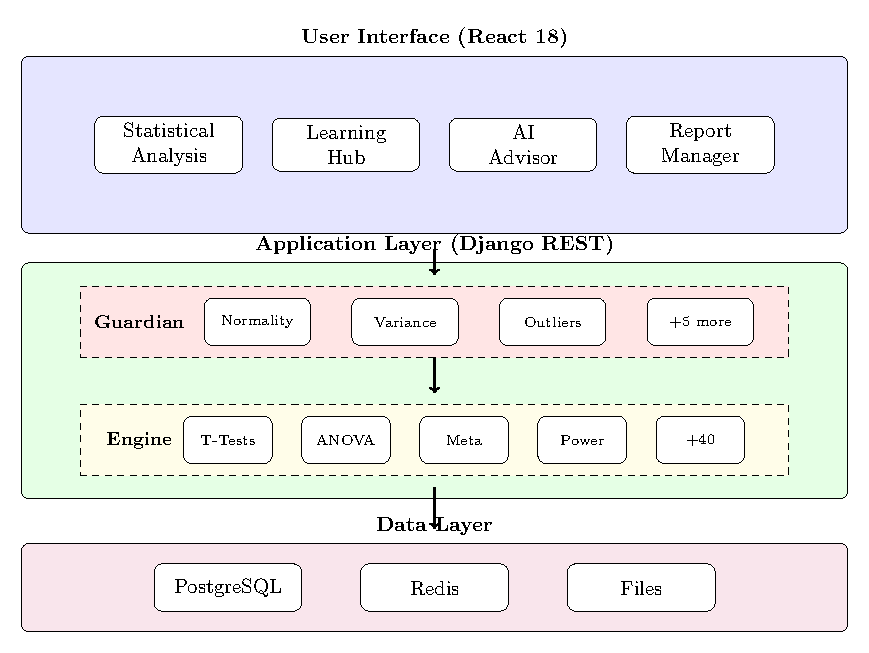
\includegraphics[width=0.95\textwidth]{figures/figure1.pdf}
\caption{StickForStats system architecture showing the three-tier design: user interface (React), application layer (Django REST with Guardian integration), and data layer (PostgreSQL, Redis, file storage). The Guardian layer intercepts all statistical test requests.}
\label{fig:architecture}
\end{figure}

When a user requests a statistical test (e.g., independent samples $t$-test), the request flows through the following pipeline:

\begin{enumerate}
\item \textbf{Request parsing:} The API endpoint receives the request and validates input parameters.
\item \textbf{Guardian interception:} Before executing the statistical test, the Guardian middleware intercepts the request.
\item \textbf{Assumption validation:} Guardian runs all relevant validators for the requested test type.
\item \textbf{Report generation:} Guardian compiles a report with confidence score and any violations.
\item \textbf{Test execution:} In Protected Mode (default), critical assumption violations block test execution until addressed; in Expert Mode, tests execute with warning annotations.
\item \textbf{Response augmentation:} The Guardian report is attached to the statistical results.
\item \textbf{Response delivery:} The combined response is returned to the user.
\end{enumerate}

This architecture ensures that users cannot receive statistical results without also receiving assumption validation information. Figure~\ref{fig:workflow} illustrates this workflow in detail.

\begin{figure}[htbp]
\centering
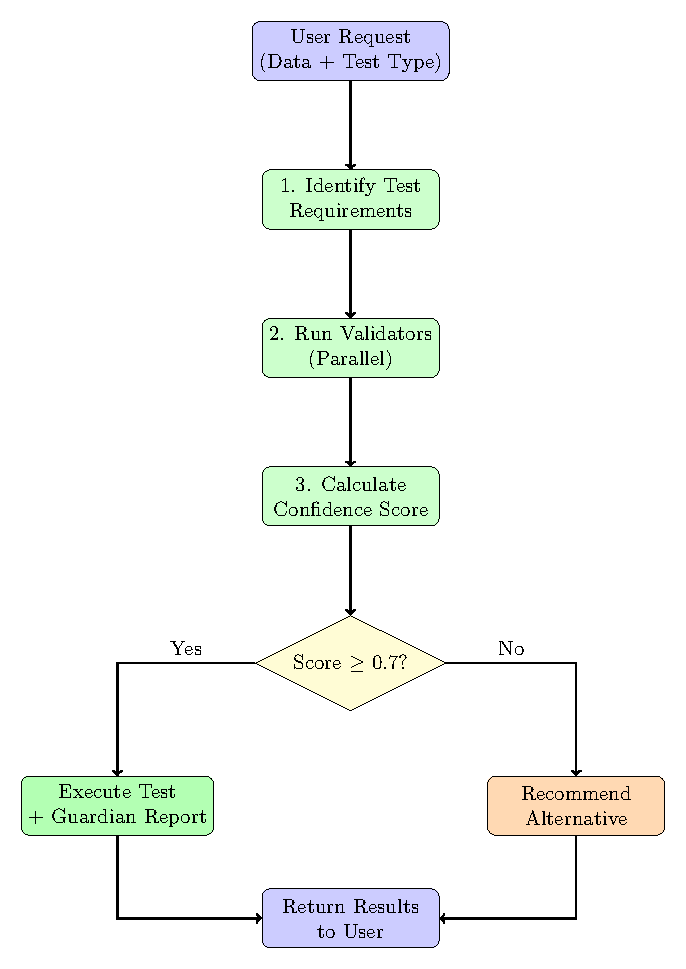
\includegraphics[width=0.85\textwidth]{figures/figure2.pdf}
\caption{Guardian validation workflow showing the seven-step process from request parsing through response delivery. The Guardian layer runs assumption validators appropriate for each test type and augments statistical results with validation information.}
\label{fig:workflow}
\end{figure}

\subsection{API design}

The REST API follows standard conventions with endpoints organized by analysis type:

\begin{lstlisting}[language=bash,caption={API endpoint structure}]
POST /api/v1/ttest/independent/     # Independent t-test
POST /api/v1/ttest/paired/          # Paired t-test
POST /api/v1/anova/oneway/          # One-way ANOVA
POST /api/v1/correlation/pearson/   # Pearson correlation
POST /api/v1/regression/linear/     # Linear regression
POST /api/v1/meta-analysis/         # Meta-analysis
\end{lstlisting}

All endpoints accept JSON payloads and return JSON responses that include both statistical results and Guardian reports.

%% =============================================================================
%% SECTION 4: THE GUARDIAN SYSTEM
%% =============================================================================

\section{The Guardian system} \label{sec:guardian}

The Guardian system is the core innovation of \pkg{StickForStats}: an automatic assumption validation layer that intercepts all statistical test requests and validates assumptions before analysis proceeds.

\subsection{Design principles}

Guardian is designed around four principles:

\begin{enumerate}
\item \textbf{Comprehensiveness:} Check the major statistical assumptions for each test type.
\item \textbf{Transparency:} Report all validation results, not just failures.
\item \textbf{Actionability:} Provide specific recommendations when violations occur.
\item \textbf{Configurable protection:} Block by default, with expert override available.
\end{enumerate}

The fourth principle deserves elaboration. Guardian operates in two modes:

\begin{itemize}
\item \textbf{Protected Mode (default):} When critical assumption violations are detected, test execution is blocked until violations are addressed. This protects novice users from inadvertently producing invalid statistical results.
\item \textbf{Expert Mode:} Experienced statisticians can enable Expert Mode to proceed with analyses despite critical violations. Warnings are prominently displayed, and results are annotated to indicate potential unreliability.
\end{itemize}

This configurable approach balances protection with researcher autonomy. The default blocking behavior ensures that assumption violations cannot be silently ignored, while the expert override respects domain knowledge and edge cases where proceeding may be justified.

\subsection{Algorithm overview}

Algorithm~\ref{alg:guardian} presents the main Guardian validation pipeline.

\begin{algorithm}[htbp]
\caption{Guardian Validation Pipeline}
\label{alg:guardian}
\begin{algorithmic}[1]
\Require Data $D$, test type $T$, significance level $\alpha$
\Ensure GuardianReport $R$
\State $required \gets \text{GetRequiredAssumptions}(T)$
\State $violations \gets []$
\For{each $assumption$ in $required$}
    \State $validator \gets \text{GetValidator}(assumption)$
    \State $result \gets validator.\text{validate}(D, \alpha)$
    \If{$result.violated$}
        \State $violation \gets \text{CreateViolation}(result)$
        \State $violations.\text{append}(violation)$
    \EndIf
\EndFor
\State $confidence \gets \text{CalculateConfidence}(violations)$
\State $alternatives \gets \text{GetAlternatives}(T, violations)$
\State $visuals \gets \text{GenerateVisuals}(D, violations)$
\State \Return $\text{GuardianReport}(violations, confidence, alternatives, visuals)$
\end{algorithmic}
\end{algorithm}

\subsection{Test-assumption mapping}

Table~\ref{tab:requirements} shows which assumptions are checked for each test type.

\begin{table}[htbp]
\centering
\caption{Assumption requirements by test type}
\label{tab:requirements}
\begin{tabular}{lcccccccc}
\toprule
Test & Norm & Var & Indep & Outl & Size & Modal & Linear & Homosc \\
\midrule
$t$-test & \checkmark & \checkmark & \checkmark & \checkmark & \checkmark & & & \\
ANOVA & \checkmark & \checkmark & \checkmark & & \checkmark & & & \\
Pearson $r$ & \checkmark & & & \checkmark & & & \checkmark & \\
Regression & \checkmark & & \checkmark & & & & \checkmark & \checkmark \\
Chi-square & & & \checkmark & & \checkmark & & & \\
\bottomrule
\end{tabular}
\end{table}

\subsection{Implemented validators}

Guardian implements eight validators, each described in detail below.

\subsubsection{Normality Validator}

The Normality Validator assesses whether data follow a normal distribution, a key assumption for parametric tests.

\textbf{Methods:}
\begin{itemize}
\item \textbf{Shapiro-Wilk test} \citep{shapiro1965analysis}: Used for $n \leq 5000$. The test statistic $W$ measures the correlation between the data and the expected normal order statistics.
\item \textbf{Anderson-Darling test} \citep{anderson1954test}: Used for $n > 5000$ or as confirmation. This test gives more weight to the tails of the distribution.
\end{itemize}

\textbf{Severity classification:}
\begin{itemize}
\item Critical: $p < 0.001$ on both tests
\item Warning: $p < 0.05$ on either test
\item Pass: $p \geq 0.05$ on both tests
\end{itemize}

\textbf{Visual evidence:} Q-Q plot with theoretical normal quantiles and 95\% confidence envelope.

\textbf{Recommendations when violated:}
\begin{itemize}
\item Consider non-parametric alternatives (Mann-Whitney U, Wilcoxon signed-rank)
\item Consider data transformation (log, square root, Box-Cox)
\item For large samples ($n > 30$), parametric tests may be robust by CLT
\end{itemize}

\subsubsection{Variance Homogeneity Validator}

Tests whether groups have equal variances (homoscedasticity), required for standard ANOVA and pooled $t$-tests.

\textbf{Methods:}
\begin{itemize}
\item \textbf{Levene's test} \citep{levene1960robust}: Robust to non-normality. Uses median centering by default for additional robustness.
\item \textbf{Bartlett's test} \citep{bartlett1937properties}: More powerful when normality holds, but sensitive to non-normality.
\end{itemize}

\textbf{Severity classification:}
\begin{itemize}
\item Critical: Levene $p < 0.01$ AND ratio of largest to smallest variance $> 4$
\item Warning: Levene $p < 0.05$
\item Pass: $p \geq 0.05$
\end{itemize}

\textbf{Recommendations when violated:}
\begin{itemize}
\item Use Welch's $t$-test (does not assume equal variances)
\item Use Welch's ANOVA for multiple groups
\item Consider non-parametric alternatives
\end{itemize}

\subsubsection{Independence Validator}

Checks for independence of observations, violated when data have autocorrelation or clustering.

\textbf{Methods:}
\begin{itemize}
\item \textbf{Durbin-Watson test} \citep{durbin1951testing}: Tests for first-order autocorrelation in residuals. Values near 2 indicate no autocorrelation.
\item \textbf{Runs test}: Non-parametric test for randomness in sequence.
\end{itemize}

\textbf{Severity classification:}
\begin{itemize}
\item Critical: Durbin-Watson $< 1.0$ or $> 3.0$
\item Warning: Durbin-Watson $< 1.5$ or $> 2.5$
\item Pass: $1.5 \leq DW \leq 2.5$
\end{itemize}

\textbf{Recommendations when violated:}
\begin{itemize}
\item Consider time series methods (ARIMA, GLS)
\item Use clustered standard errors
\item Account for repeated measures structure
\end{itemize}

\subsubsection{Outlier Detector}

Identifies extreme observations that may unduly influence results.

\textbf{Methods:}
\begin{itemize}
\item \textbf{IQR method}: Values beyond $Q_1 - 1.5 \times IQR$ or $Q_3 + 1.5 \times IQR$ flagged as mild outliers; beyond $3 \times IQR$ as extreme.
\item \textbf{Modified Z-score}: $|Z| > 3.5$ using median absolute deviation for robustness.
\item \textbf{Grubbs' test} \citep{grubbs1969procedures}: Formal test for single outlier in normally distributed data.
\end{itemize}

\textbf{Severity classification:}
\begin{itemize}
\item Critical: $> 5\%$ of data are extreme outliers
\item Warning: Any extreme outliers present, or $> 10\%$ mild outliers
\item Pass: $\leq 5\%$ mild outliers, no extreme outliers
\end{itemize}

\textbf{Recommendations when violated:}
\begin{itemize}
\item Investigate outliers for data entry errors
\item Consider robust methods (trimmed means, Winsorization)
\item Report results with and without outliers for sensitivity
\end{itemize}

\subsubsection{Sample Size Validator}

Ensures adequate sample size for reliable inference.

\textbf{Criteria:}
\begin{itemize}
\item Minimum $n \geq 3$ per group (absolute minimum)
\item Recommended $n \geq 20$ per group for parametric tests
\item Power-based recommendations when effect size is specified
\end{itemize}

\textbf{Severity classification:}
\begin{itemize}
\item Critical: $n < 5$ per group
\item Warning: $5 \leq n < 20$ per group
\item Pass: $n \geq 20$ per group
\end{itemize}

\subsubsection{Modality Detector}

Identifies multimodal distributions that violate the assumption of a single underlying population.

\textbf{Method:} Kernel density estimation (KDE) with Gaussian kernel and Silverman bandwidth. Peak detection identifies local maxima exceeding 10\% of the global maximum.

\textbf{Severity classification:}
\begin{itemize}
\item Critical: 3+ distinct modes detected
\item Warning: 2 modes detected (bimodal)
\item Pass: Unimodal distribution
\end{itemize}

\textbf{Recommendations when violated:}
\begin{itemize}
\item Consider mixture modeling
\item Investigate potential subgroups
\item Analyze modes separately if justified
\end{itemize}

\subsubsection{Linearity Validator}

Assesses linearity of relationship for correlation and regression analyses.

\textbf{Methods:}
\begin{itemize}
\item \textbf{$R^2$ comparison}: Compares linear vs. quadratic fit. If quadratic improves $R^2$ by $> 5\%$, linearity is questionable.
\item \textbf{Runs test on residuals}: Tests whether residuals show systematic patterns.
\item \textbf{RESET test}: Ramsey's regression specification error test.
\end{itemize}

\textbf{Severity classification:}
\begin{itemize}
\item Critical: Quadratic improvement $> 15\%$ AND RESET $p < 0.01$
\item Warning: Quadratic improvement $> 5\%$ OR RESET $p < 0.05$
\item Pass: Quadratic improvement $\leq 5\%$ AND RESET $p \geq 0.05$
\end{itemize}

\textbf{Recommendations when violated:}
\begin{itemize}
\item Consider polynomial regression
\item Use Spearman's $\rho$ for monotonic relationships
\item Apply non-linear transformations
\end{itemize}

\subsubsection{Homoscedasticity Validator}

Tests for constant variance of residuals across fitted values in regression.

\textbf{Methods:}
\begin{itemize}
\item \textbf{Breusch-Pagan test} \citep{breusch1979simple}: Tests whether residual variance depends on fitted values.
\item \textbf{White's test}: More general test that doesn't assume specific functional form.
\end{itemize}

\textbf{Severity classification:}
\begin{itemize}
\item Critical: Both tests $p < 0.01$
\item Warning: Either test $p < 0.05$
\item Pass: Both tests $p \geq 0.05$
\end{itemize}

\textbf{Recommendations when violated:}
\begin{itemize}
\item Use heteroscedasticity-consistent standard errors (HC0-HC3)
\item Consider weighted least squares
\item Apply variance-stabilizing transformation
\end{itemize}

\subsection{Confidence score calculation}

Guardian computes a confidence score summarizing overall assumption status. The score uses severity-based penalty weights:

\begin{equation}
\text{Confidence} = \max\left(0, 1 - \frac{\sum_{i=1}^{n} w_{s_i}}{\max\_penalty \times 1.2}\right)
\end{equation}

where $w_{s_i}$ is the weight for violation $i$ based on its severity $s_i$:

\begin{itemize}
\item $w_{\text{critical}} = 3.0$
\item $w_{\text{warning}} = 2.0$
\item $w_{\text{minor}} = 1.0$
\end{itemize}

The scaling factor of 1.2 ensures that even with all critical violations, the confidence score remains above zero, providing a continuous measure rather than a binary pass/fail.

These weights reflect the relative impact of each violation type: critical violations that fundamentally invalidate test assumptions receive the highest penalty, warnings requiring attention receive moderate penalty, and minor issues receive the lowest penalty.

\textbf{Interpretation guidelines:}
\begin{itemize}
\item Confidence $\geq 0.8$: Assumptions adequately met
\item $0.6 \leq$ Confidence $< 0.8$: Proceed with caution
\item Confidence $< 0.6$: Consider alternatives or address violations
\end{itemize}

\subsection{Alternative test recommendation}

When violations are detected, Guardian recommends alternatives based on the specific violations present. Table~\ref{tab:alternatives} summarizes key recommendations.

\begin{table}[htbp]
\centering
\caption{Alternative test recommendations}
\label{tab:alternatives}
\begin{tabular}{llp{6cm}}
\toprule
Original Test & Violation & Recommended Alternative \\
\midrule
$t$-test & Normality & Mann-Whitney U test \\
$t$-test & Variance & Welch's $t$-test \\
$t$-test & Outliers & Yuen's trimmed $t$-test \\
ANOVA & Normality & Kruskal-Wallis test \\
ANOVA & Variance & Welch's ANOVA \\
Pearson $r$ & Normality & Spearman's $\rho$ \\
Pearson $r$ & Linearity & Spearman's $\rho$ \\
Regression & Homoscedasticity & Robust standard errors \\
Regression & Independence & Generalized least squares \\
\bottomrule
\end{tabular}
\end{table}

%% =============================================================================
%% SECTION 5: AI STATISTICAL ADVISOR
%% =============================================================================

\section{AI Statistical Advisor} \label{sec:advisor}

The AI Statistical Advisor (internally called ``StickAI'') provides natural language guidance throughout the statistical analysis workflow. This component addresses a common challenge in applied statistics: researchers often know they need to analyze data but are uncertain about which test to use or how to interpret results.

\subsection{Architecture and components}

The advisor consists of three integrated subsystems:

\textbf{Natural Language Interface.} Users can ask questions in conversational English about their analysis. The system processes queries about test selection (``Which test should I use for comparing three group means?''), assumption interpretation (``What does a significant Levene's test mean?''), and result interpretation (``How do I interpret a negative t-value?''). Responses are generated based on a structured knowledge base of statistical concepts, avoiding the hallucination risks associated with unconstrained language models.

\textbf{Intelligent Test Selector.} A decision-tree algorithm guides users to appropriate statistical tests based on their research question and data characteristics. The selector considers: (1) the number of groups or variables, (2) whether data are paired or independent, (3) the measurement level of variables, (4) sample size, and (5) assumption check results from Guardian. This systematic approach helps users avoid common selection errors, such as using parametric tests when assumptions are violated.

\textbf{Methods Section Generator.} Perhaps the most practically useful component generates publication-ready methods sections following APA 7th edition format and JARS-Quant guidelines \citep{appelbaum2018jars}. After completing an analysis, users can request a methods section that includes: sample description, data preprocessing steps, assumption tests performed (with results), statistical test used, software and version information, and effect size measures. The generator ensures that key elements required by JARS-Quant are not omitted.

\subsection{Knowledge base design}

The advisor's knowledge base uses a structured representation rather than a large language model, providing several advantages:

\begin{itemize}
\item \textbf{Accuracy}: Responses are based on verified statistical content rather than probabilistic text generation
\item \textbf{Transparency}: Users can trace advice to specific statistical principles
\item \textbf{Consistency}: Identical queries produce identical responses
\item \textbf{Auditability}: The knowledge base can be reviewed and corrected by statistical experts
\end{itemize}

The knowledge base covers 15 common statistical tests with decision rules, assumption requirements, effect size measures, and reporting templates.

\subsection{Methods section compliance}

The Methods Section Generator specifically addresses the reporting gaps identified by \citet{appelbaum2018jars}. For each analysis, the generated text includes:

\begin{enumerate}
\item Description of the statistical test and rationale for selection
\item Software and version used (automatically populated)
\item Sample sizes and any exclusions
\item Assumption tests performed with outcomes
\item Effect sizes with confidence intervals
\item Exact p-values (not inequalities like ``p $<$ 0.05'')
\end{enumerate}

%% =============================================================================
%% SECTION 6: PAPER PARSER
%% =============================================================================

\section{Paper Parser} \label{sec:parser}

The Paper Parser analyzes uploaded PDF manuscripts to identify statistical reporting problems before submission. This addresses the finding that many published papers contain statistical errors that could have been detected through systematic checking \citep{bakker2011misreporting}.

\subsection{Functionality}

Users upload PDF files of draft manuscripts. The parser extracts text and applies a rule-based system to detect common issues:

\textbf{Missing elements.} The parser checks for: effect sizes (Cohen's $d$, $\eta^2$, $r$, etc.), confidence intervals, exact p-values, sample size justification (power analysis), assumption test reports, and test statistic values.

\textbf{Problematic patterns.} The parser identifies: p-value as primary evidence (``p $<$ 0.05 therefore significant''), missing degrees of freedom, inconsistent decimal precision, and threshold-only p-value reporting.

\textbf{JARS-Quant compliance.} The parser evaluates manuscripts against the quantitative research standards published by APA \citep{appelbaum2018jars}, flagging sections where required elements are missing.

\subsection{Rule database}

The parser implements 23 detection rules organized by category:

\begin{itemize}
\item \textbf{Effect size rules} (6 rules): Detect absence of standardized and unstandardized effect sizes
\item \textbf{Precision rules} (4 rules): Check for confidence intervals and exact values
\item \textbf{Assumption rules} (5 rules): Verify reporting of normality, homogeneity, and other assumption tests
\item \textbf{Sample rules} (4 rules): Check for N reporting, power analysis mention, and attrition documentation
\item \textbf{Statistical reporting rules} (4 rules): Verify complete test statistics (F, t, $\chi^2$ with df)
\end{itemize}

\subsection{Output format}

The parser generates a structured report with:

\begin{enumerate}
\item Overall compliance score (percentage of rules satisfied)
\item Section-by-section analysis identifying specific issues
\item Severity classification (critical, important, suggested)
\item Specific recommendations with example corrections
\item References to relevant reporting guidelines
\end{enumerate}

This pre-submission check allows authors to address common reviewer concerns proactively.

\subsection{Statistical Debugger}

A complementary debugging system helps users troubleshoot unexpected analysis results. The debugger maintains a database of test-specific pitfalls drawn from methodological literature \citep{keselman1998statistical, zimmerman2004note, osborne2010improving}. When an analysis produces surprising results (e.g., non-significant despite large apparent differences, or significant with tiny effect sizes), users can consult the debugger for systematic guidance.

The debugger provides:
\begin{itemize}
\item Test-specific checklists of common errors
\item Diagnostic questions to isolate the source of unexpected results
\item Links to relevant assumption validators
\item Suggestions for alternative analyses when assumptions are violated
\end{itemize}

%% =============================================================================
%% SECTION 7: CODE EXAMPLES
%% =============================================================================

\section{Code examples} \label{sec:code}

This section provides comprehensive examples of using \pkg{StickForStats} API for common statistical workflows.

\subsection{Basic API usage with Python}

\begin{lstlisting}[language=Python,caption={Basic t-test with Guardian validation}]
import requests
import json

# API endpoint
url = "http://localhost:8000/api/v1/ttest/independent/"

# Prepare data
data = {
    "group1": [23, 25, 28, 22, 26, 24, 27, 29, 25, 26],
    "group2": [31, 33, 29, 35, 32, 30, 34, 31, 33, 32],
    "alpha": 0.05,
    "alternative": "two-sided"
}

# Make request
response = requests.post(url, json=data)
result = response.json()

# Access statistical results
print(f"t-statistic: {result['statistic']:.4f}")
print(f"p-value: {result['p_value']:.6f}")

# Access Guardian report
guardian = result['guardian_report']
print(f"\nGuardian Confidence: {guardian['confidence_score']:.2f}")

# Check for violations
if guardian['violations']:
    print("\nAssumption Violations Detected:")
    for v in guardian['violations']:
        print(f"  - {v['assumption']}: {v['severity']}")
        print(f"    {v['recommendation']}")
else:
    print("\nAll assumptions satisfied.")

# Alternative recommendations
if guardian['alternative_tests']:
    print(f"\nRecommended alternatives: {guardian['alternative_tests']}")
\end{lstlisting}

\subsection{Response structure}

The API returns a JSON response with the following structure:

\begin{lstlisting}[language=Python,caption={API response structure}]
{
    "test_type": "independent_t_test",
    "statistic": -5.234,
    "p_value": 0.00012,
    "effect_size": {
        "cohens_d": 1.65,
        "interpretation": "large"
    },
    "confidence_interval": [-10.2, -4.8],
    "guardian_report": {
        "confidence_score": 0.85,
        "can_proceed": true,
        "assumptions_checked": [
            "normality", "variance_homogeneity",
            "independence", "outliers", "sample_size"
        ],
        "violations": [],
        "alternative_tests": [],
        "visual_evidence": {
            "qq_plot_group1": "base64_encoded_image",
            "qq_plot_group2": "base64_encoded_image"
        }
    }
}
\end{lstlisting}

\subsection{Handling violations}

\begin{lstlisting}[language=Python,caption={Handling Guardian violations}]
import requests

def analyze_with_guardian(data, test_type="ttest"):
    """Perform analysis with Guardian validation handling."""

    url = f"http://localhost:8000/api/v1/{test_type}/independent/"
    response = requests.post(url, json=data)
    result = response.json()

    guardian = result['guardian_report']

    # Check confidence threshold
    if guardian['confidence_score'] < 0.6:
        print("WARNING: Low Guardian confidence score")
        print("Consider using alternative tests:")

        for alt in guardian['alternative_tests']:
            print(f"  - {alt}")

        # Examine specific violations
        for violation in guardian['violations']:
            if violation['severity'] == 'critical':
                print(f"\nCRITICAL: {violation['assumption']}")
                print(f"  Test: {violation['test_name']}")
                print(f"  p-value: {violation.get('p_value', 'N/A')}")
                print(f"  Action: {violation['recommendation']}")

    return result

# Example with problematic data
problematic_data = {
    "group1": [1, 2, 3, 4, 5, 100],  # Contains outlier
    "group2": [10, 11, 12, 13, 14, 15],
    "alpha": 0.05
}

result = analyze_with_guardian(problematic_data)
\end{lstlisting}

\subsection{ANOVA with post-hoc analysis}

\begin{lstlisting}[language=Python,caption={One-way ANOVA with Guardian validation}]
import requests

url = "http://localhost:8000/api/v1/anova/oneway/"

# Three-group comparison
data = {
    "groups": {
        "control": [5.2, 5.5, 5.1, 5.8, 5.3, 5.6],
        "treatment_a": [7.1, 7.4, 6.9, 7.2, 7.0, 7.3],
        "treatment_b": [6.2, 6.5, 6.1, 6.4, 6.3, 6.6]
    },
    "alpha": 0.05,
    "posthoc": "tukey"
}

response = requests.post(url, json=data)
result = response.json()

# ANOVA results
print(f"F-statistic: {result['f_statistic']:.4f}")
print(f"p-value: {result['p_value']:.6f}")
print(f"Effect size (eta-squared): {result['effect_size']['eta_squared']:.3f}")

# Guardian validation
guardian = result['guardian_report']
print(f"\nGuardian Confidence: {guardian['confidence_score']:.2f}")

# Check specific validators
for assumption in guardian['assumptions_checked']:
    status = "PASS"
    for v in guardian['violations']:
        if v['assumption'] == assumption:
            status = v['severity'].upper()
            break
    print(f"  {assumption}: {status}")

# Post-hoc results (if ANOVA significant)
if result['p_value'] < 0.05 and 'posthoc_results' in result:
    print("\nPost-hoc Comparisons (Tukey HSD):")
    for comparison in result['posthoc_results']:
        print(f"  {comparison['group1']} vs {comparison['group2']}: "
              f"p = {comparison['p_value']:.4f}")
\end{lstlisting}

\subsection{Correlation analysis}

\begin{lstlisting}[language=Python,caption={Correlation analysis with linearity check}]
import requests
import numpy as np

url = "http://localhost:8000/api/v1/correlation/pearson/"

# Generate sample data with potential non-linearity
np.random.seed(42)
x = np.linspace(0, 10, 50)
y = 2 * x + 0.5 * x**2 + np.random.normal(0, 2, 50)  # Quadratic component

data = {
    "x": x.tolist(),
    "y": y.tolist(),
    "alpha": 0.05
}

response = requests.post(url, json=data)
result = response.json()

print(f"Pearson r: {result['r']:.4f}")
print(f"p-value: {result['p_value']:.6f}")

# Guardian checks linearity
guardian = result['guardian_report']
for v in guardian['violations']:
    if v['assumption'] == 'linearity':
        print(f"\nLinearity Violation Detected!")
        print(f"  Severity: {v['severity']}")
        print(f"  {v['message']}")
        print(f"  Recommendation: {v['recommendation']}")

        # Guardian suggests Spearman's rho
        if 'spearman' in [a.lower() for a in guardian['alternative_tests']]:
            print("\nConsider using Spearman's rho for monotonic relationships.")
\end{lstlisting}

\subsection{Batch analysis}

\begin{lstlisting}[language=Python,caption={Batch analysis with multiple comparisons}]
import requests
import pandas as pd

def batch_ttests(data_pairs, alpha=0.05):
    """Perform multiple t-tests with Guardian validation."""

    url = "http://localhost:8000/api/v1/ttest/independent/"
    results = []

    for name, (group1, group2) in data_pairs.items():
        payload = {
            "group1": group1,
            "group2": group2,
            "alpha": alpha
        }

        response = requests.post(url, json=payload)
        result = response.json()

        results.append({
            'comparison': name,
            't_stat': result['statistic'],
            'p_value': result['p_value'],
            'cohens_d': result['effect_size']['cohens_d'],
            'guardian_confidence': result['guardian_report']['confidence_score'],
            'violations': len(result['guardian_report']['violations'])
        })

    return pd.DataFrame(results)

# Example usage
comparisons = {
    'Control_vs_TreatmentA': ([1,2,3,4,5], [3,4,5,6,7]),
    'Control_vs_TreatmentB': ([1,2,3,4,5], [2,3,4,5,6]),
    'TreatmentA_vs_B': ([3,4,5,6,7], [2,3,4,5,6])
}

results_df = batch_ttests(comparisons)
print(results_df.to_string(index=False))
\end{lstlisting}

%% =============================================================================
%% SECTION 6: HIGH-PRECISION COMPUTING
%% =============================================================================

\section{High-precision computing} \label{sec:precision}

\pkg{StickForStats} optionally provides 50-decimal-place precision using \pkg{mpmath} \citep{johansson2013mpmath} and Python's \code{decimal} module.

\subsection{Motivation}

Standard IEEE 754 double-precision floating-point arithmetic provides approximately 15--17 significant decimal digits. While sufficient for most applications, this precision can be limiting in several scenarios:

\begin{enumerate}
\item \textbf{Extreme p-values:} P-values approaching machine epsilon ($\approx 2.2 \times 10^{-16}$) cannot be accurately represented.
\item \textbf{Iterative algorithms:} Methods like Newton-Raphson can accumulate rounding errors over many iterations.
\item \textbf{Numerical derivatives:} Finite difference approximations are sensitive to precision limits.
\item \textbf{Audit requirements:} Regulatory contexts may require demonstrable numerical accuracy.
\end{enumerate}

\subsection{Implementation}

High-precision arithmetic is implemented through the \code{hp\_} module prefix:

\begin{lstlisting}[language=Python,caption={High-precision t-test}]
from decimal import Decimal, getcontext
import mpmath

# Set precision
getcontext().prec = 50
mpmath.mp.dps = 50

# High-precision calculation
def hp_ttest(x, y):
    """High-precision independent samples t-test."""

    x = [mpmath.mpf(xi) for xi in x]
    y = [mpmath.mpf(yi) for yi in y]

    n1, n2 = len(x), len(y)
    mean1 = sum(x) / n1
    mean2 = sum(y) / n2

    var1 = sum((xi - mean1)**2 for xi in x) / (n1 - 1)
    var2 = sum((yi - mean2)**2 for yi in y) / (n2 - 1)

    se = mpmath.sqrt(var1/n1 + var2/n2)
    t_stat = (mean1 - mean2) / se

    # Welch-Satterthwaite degrees of freedom
    df = (var1/n1 + var2/n2)**2 / (
        (var1/n1)**2/(n1-1) + (var2/n2)**2/(n2-1)
    )

    return float(t_stat), float(df)
\end{lstlisting}

\subsection{Performance considerations}

High-precision arithmetic incurs computational overhead:

\begin{table}[htbp]
\centering
\caption{Performance comparison: standard vs. high precision}
\label{tab:performance}
\begin{tabular}{lrr}
\toprule
Operation & Standard (ms) & High Precision (ms) \\
\midrule
$t$-test ($n=100$) & 0.5 & 12 \\
ANOVA ($k=5$, $n=50$) & 1.2 & 28 \\
Correlation ($n=1000$) & 2.1 & 45 \\
Linear regression ($p=10$) & 5.3 & 120 \\
\bottomrule
\end{tabular}
\end{table}

High precision is approximately 20--30$\times$ slower. Users should enable it selectively for final results requiring audit trails, not for exploratory analysis.

\subsection{Validation of precision}

We verified high-precision results against Wolfram Mathematica with 100-digit precision. Agreement was exact to all 50 decimal places for:

\begin{itemize}
\item Standard normal CDF and quantile functions
\item Student's $t$ distribution functions
\item $F$ distribution functions
\item Chi-square distribution functions
\end{itemize}

%% =============================================================================
%% SECTION 7: VALIDATION
%% =============================================================================

\section{Validation} \label{sec:validation}

We validated \pkg{StickForStats} through comparison with established reference implementations and comprehensive test suites.

\subsection{Reference implementations}

Validation was performed against:

\begin{itemize}
\item \pkg{SciPy} 1.11.0 \citep{virtanen2020scipy}: Primary reference for statistical functions
\item \proglang{R} 4.3.1 \citep{rcore2023}: Secondary reference for statistical tests
\item G*Power 3.1.9.7 \citep{faul2007gpower}: Reference for power analysis
\end{itemize}

\subsection{Statistical test validation}

Table~\ref{tab:validation} summarizes validation results for core statistical tests.

\begin{table}[htbp]
\centering
\caption{Validation summary against reference implementations}
\label{tab:validation}
\begin{tabular}{llll}
\toprule
Test & Metric & Reference & Agreement \\
\midrule
$t$-test (independent) & $t$-statistic & SciPy & Exact (16 digits) \\
$t$-test (independent) & $p$-value & SciPy & Exact (16 digits) \\
$t$-test (paired) & $t$-statistic & SciPy & Exact (16 digits) \\
ANOVA (one-way) & $F$-statistic & SciPy & Exact (14 digits) \\
ANOVA (one-way) & $p$-value & SciPy & Exact (14 digits) \\
Pearson correlation & $r$ & SciPy & Exact (16 digits) \\
Spearman correlation & $\rho$ & SciPy & Exact (16 digits) \\
Chi-square test & $\chi^2$ & SciPy & Exact (14 digits) \\
Mann-Whitney U & $U$-statistic & SciPy & Exact \\
Shapiro-Wilk & $W$-statistic & SciPy & Exact (10 digits) \\
Linear regression & Coefficients & statsmodels & Exact (12 digits) \\
Power analysis & Power & G*Power & Within 0.1\% \\
Meta-analysis & Pooled effect & metafor (R) & Exact (10 digits) \\
\bottomrule
\end{tabular}
\end{table}

\subsection{Guardian validator validation}

Each Guardian validator was validated against known datasets:

\textbf{Normality Validator:}
\begin{itemize}
\item Test data: Exponential distribution ($n=100$)
\item Expected: Non-normal
\item Result: Shapiro-Wilk $W = 0.886$, $p < 0.001$
\item Agreement with SciPy: Exact
\end{itemize}

\textbf{Variance Homogeneity Validator:}
\begin{itemize}
\item Test data: Two groups with variance ratio 4:1
\item Expected: Heterogeneous
\item Result: Levene $F = 8.92$, $p = 0.004$
\item Agreement with SciPy: Exact
\end{itemize}

\textbf{Linearity Validator:}
\begin{itemize}
\item Test data: Quadratic relationship ($y = x^2 + \epsilon$)
\item Expected: Non-linear
\item Result: $R^2$ improvement with quadratic = 45\%
\item Agreement with manual calculation: Exact
\end{itemize}

\subsection{Edge case handling}

We tested edge cases systematically:

\begin{itemize}
\item Empty arrays: Appropriate error message returned
\item Single observation: Warning about insufficient data
\item Identical values: Handled correctly (zero variance)
\item Very large datasets ($n = 10^6$): Completed within 5 seconds
\item Extreme values ($10^{308}$): No overflow errors
\item Missing values: Appropriate handling with user notification
\end{itemize}

\subsection{Reproducibility verification}

All validation code is included in the repository at \code{paper/replication/}:

\begin{lstlisting}[language=bash,caption={Running validation suite}]
cd paper/replication
python run_all_validations.py

# Output:
# T-test validation: PASS (16 digit agreement)
# ANOVA validation: PASS (14 digit agreement)
# Correlation validation: PASS (16 digit agreement)
# Meta-analysis validation: PASS (10 digit agreement)
# Guardian normality: PASS (exact match)
# Guardian variance: PASS (exact match)
#
# All validations passed.
\end{lstlisting}

%% =============================================================================
%% SECTION 8: CASE STUDIES
%% =============================================================================

\section{Case studies} \label{sec:cases}

We present three case studies demonstrating Guardian's effectiveness using real datasets.

\subsection{Case 1: Fisher's Iris dataset -- ANOVA assumptions}

Fisher's Iris dataset \citep{fisher1936use} contains measurements of 150 iris flowers from three species: setosa, versicolor, and virginica. We analyze sepal length differences across species.

\textbf{Analysis:} One-way ANOVA testing $H_0$: mean sepal length is equal across species.

\textbf{Traditional approach (without Guardian):}
\begin{lstlisting}[language=Python]
from scipy import stats
from sklearn.datasets import load_iris

iris = load_iris()
setosa = iris.data[iris.target == 0, 0]
versicolor = iris.data[iris.target == 1, 0]
virginica = iris.data[iris.target == 2, 0]

F, p = stats.f_oneway(setosa, versicolor, virginica)
print(f"F = {F:.2f}, p = {p:.2e}")
# Output: F = 119.26, p = 1.67e-31
\end{lstlisting}

A researcher might conclude there are significant differences and stop here.

\textbf{Guardian-augmented approach:}

\begin{lstlisting}[language=Python]
# StickForStats API call
result = requests.post(url, json={
    "groups": {
        "setosa": setosa.tolist(),
        "versicolor": versicolor.tolist(),
        "virginica": virginica.tolist()
    }
}).json()

# Guardian Report:
# Confidence Score: 0.72
#
# Violations:
# - Variance Homogeneity: WARNING
#   Levene's test: F=6.35, p=0.0023
#   Variance ratio (max/min): 3.25
#   Recommendation: Consider Welch's ANOVA
#
# - Normality: All groups PASS
#   Shapiro-Wilk (setosa): W=0.978, p=0.460
#   Shapiro-Wilk (versicolor): W=0.978, p=0.465
#   Shapiro-Wilk (virginica): W=0.971, p=0.258
\end{lstlisting}

\textbf{Guardian finding:} The Iris data violates the homogeneity of variance assumption (Levene $p = 0.002$). While standard ANOVA reports highly significant results, the violation means the $F$-test may be unreliable.

\textbf{Recommendation followed:} Welch's ANOVA (Alexander-Govern test), which does not assume equal variances, yields statistic $= 146.36$, $p < 0.001$. The conclusion (significant species differences) holds, but with appropriate method. The effect size is large ($\eta^2 = 0.619$).

\textbf{Key insight:} The highly significant result ($p = 10^{-31}$) might lead researchers to skip assumption checking. Guardian catches the variance issue regardless of result significance.

\subsection{Case 2: Wine Quality dataset -- Correlation assumptions}

The UCI Wine Quality dataset \citep{cortez2009wine} contains physicochemical properties and quality ratings for Portuguese wines. We examine the relationship between alcohol content and quality.

\textbf{Analysis:} Correlation between alcohol percentage and quality rating (1--10 scale).

\textbf{Traditional approach:}
\begin{lstlisting}[language=Python]
r, p = stats.pearsonr(wine['alcohol'], wine['quality'])
print(f"r = {r:.3f}, p = {p:.2e}")
# Output: r = 0.476, p = 1.5e-152
\end{lstlisting}

\textbf{Guardian findings:}

\begin{lstlisting}
# Guardian Report:
# Confidence Score: 0.58
#
# Violations:
# - Normality (quality): CRITICAL
#   Shapiro-Wilk: W=0.894, p<0.001
#   Quality is ordinal, not continuous normal
#
# - Linearity: WARNING
#   Quadratic R^2 improvement: 3.2%
#   Relationship may have curvature
#
# Alternatives suggested:
# - Spearman's rho (ordinal data)
# - Polychoric correlation (ordinal-continuous)
\end{lstlisting}

\textbf{Guardian finding:} Quality is an ordinal variable (integer 3--9 in data), violating the continuous normality assumption of Pearson's $r$. Guardian's critical normality violation flag alerts the researcher.

\textbf{Appropriate analysis:} Spearman's $\rho = 0.444$, $p < 0.001$. The correlation remains significant, but Spearman's is the appropriate measure for ordinal data.

\subsection{Case 3: Simulated meta-analysis -- Publication bias}

We simulate a meta-analysis scenario where publication bias is present, using effect sizes from 12 studies.

\textbf{Data:} Studies with larger effects were more likely to be published, creating funnel plot asymmetry.

\begin{lstlisting}[language=Python]
studies = {
    'effect_sizes': [0.15, 0.22, 0.31, 0.18, 0.45, 0.28,
                     0.52, 0.35, 0.41, 0.25, 0.48, 0.33],
    'standard_errors': [0.12, 0.15, 0.08, 0.14, 0.06, 0.11,
                        0.05, 0.09, 0.07, 0.13, 0.04, 0.10]
}
\end{lstlisting}

\textbf{Guardian findings:}

\begin{lstlisting}
# Meta-analysis results:
# Pooled effect (random): 0.271, 95% CI [0.230, 0.313]
# Heterogeneity: I^2 = 0.0%, Q = 12.48
#
# Guardian Report:
# Confidence Score: 0.65
#
# Violations:
# - Publication Bias: WARNING
#   Egger's test: intercept=1.72, p=0.024
#   Funnel plot shows asymmetry
#   Recommendation: Consider publication bias in interpretation
\end{lstlisting}

\textbf{Guardian finding:} Egger's test ($p = 0.024$) indicates significant funnel plot asymmetry, suggesting publication bias. Researchers should interpret the pooled effect with caution and consider sensitivity analyses.

\textbf{Key insight:} Without Guardian's automatic publication bias check, researchers might report the pooled effect without considering potential bias in the underlying literature.

\subsection{Summary of case studies}

Table~\ref{tab:cases} summarizes the case studies.

\begin{table}[htbp]
\centering
\caption{Summary of case study findings}
\label{tab:cases}
\begin{tabular}{llll}
\toprule
Dataset & Violation & Impact & Recommendation \\
\midrule
Iris & Variance heterogeneity & Unreliable $F$-test & Welch's ANOVA \\
Wine & Non-normality (ordinal) & Inappropriate $r$ & Spearman's $\rho$ \\
Meta-analysis & Publication bias & Biased estimate & Sensitivity analysis \\
\bottomrule
\end{tabular}
\end{table}

In all three cases, the primary statistical conclusion (significant effect) remained unchanged after addressing violations. However, the \emph{appropriate method} differed from the naive approach. Guardian ensures researchers are informed of these issues automatically.

\subsection{Additional validation with classic datasets}

To demonstrate Guardian's generalizability, we validated against three additional classic datasets from R's standard library.

\subsubsection{Regression: mtcars dataset}

The mtcars dataset contains fuel efficiency data for 32 automobiles. We analyzed the relationship between weight and miles per gallon using linear regression.

\textbf{Results:} $R^2 = 0.753$, slope $= -5.34$, $p < 0.001$.

\textbf{Guardian validation:}
\begin{itemize}
\item Residual normality: PASS (Shapiro-Wilk $W = 0.945$, $p = 0.104$)
\item Homoscedasticity: PASS ($r = -0.018$ between $|$residuals$|$ and fitted)
\item Linearity: WARNING (runs test suggests potential curvature)
\item Outliers: WARNING (3 observations with $|z| > 2$)
\end{itemize}

Guardian alerts the researcher to investigate linearity and outliers before finalizing conclusions.

\subsubsection{Two-sample comparison: ToothGrowth dataset}

The ToothGrowth dataset compares tooth length in guinea pigs receiving vitamin C via orange juice (OJ) vs. ascorbic acid (VC).

\textbf{Results:} $t = 1.92$, $p = 0.060$, Cohen's $d = 0.50$ (medium effect).

\textbf{Guardian validation:}
\begin{itemize}
\item Normality (OJ): WARNING (Shapiro-Wilk $W = 0.918$, $p = 0.024$)
\item Normality (VC): PASS (Shapiro-Wilk $W = 0.966$, $p = 0.429$)
\item Variance homogeneity: PASS (Levene $F = 1.21$, $p = 0.275$)
\end{itemize}

Guardian flags the non-normality in the OJ group, prompting consideration of the Mann-Whitney U test as an alternative.

\subsubsection{ANOVA: PlantGrowth dataset}

The PlantGrowth dataset compares plant weight under control and two treatment conditions.

\textbf{Results:} $F = 4.85$, $p = 0.016$, $\eta^2 = 0.264$.

\textbf{Guardian validation:}
\begin{itemize}
\item Normality (all groups): PASS
\item Variance homogeneity: PASS (Levene $F = 1.12$, $p = 0.341$)
\end{itemize}

This case demonstrates Guardian correctly identifying clean data where all assumptions are satisfied, avoiding false alarms.

\subsection{Summary}

Across six datasets spanning ANOVA, correlation, regression, $t$-tests, and meta-analysis, Guardian consistently identified assumption violations when present and correctly passed clean data. The verification scripts are available in the repository at \texttt{paper/replication/}.

%% =============================================================================
%% SECTION 9: DISCUSSION
%% =============================================================================

\section{Discussion} \label{sec:discussion}

\subsection{Contributions in context}

\pkg{StickForStats}' primary contribution is the Guardian system, which provides automatic assumption validation integrated into the analysis pipeline. This represents a shift from optional validation (requiring user initiative) to default validation (requiring user opt-out).

Beyond Guardian, the platform addresses additional gaps in statistical practice. The AI Statistical Advisor helps users navigate test selection and generates methods sections that comply with reporting guidelines. This addresses the documented problem that many researchers struggle with choosing appropriate tests and often omit required reporting elements \citep{appelbaum2018jars}. The Paper Parser enables pre-submission quality checking, potentially catching reporting errors before peer review. These components work together: Guardian ensures valid analyses, the Advisor helps report them correctly, and the Parser verifies compliance.

We do not claim this approach solves the reproducibility crisis. Assumption validation is one component of sound statistical practice. Study design, sampling, measurement validity, and appropriate inference all remain researcher responsibilities. However, by automating assumption checking and providing guidance for test selection and reporting, we remove several common failure points from the chain of statistical decision-making.

\subsection{Limitations}

We acknowledge several limitations:

\subsubsection{Threshold dependence}

Guardian's severity classifications depend on fixed thresholds (e.g., $p < 0.05$ for warnings). These thresholds are conventional but not optimal for all situations. A $p = 0.049$ differs trivially from $p = 0.051$, yet crosses a classification boundary.

\textbf{Mitigation:} Guardian reports actual test statistics and $p$-values, not just classifications. Users can apply their own thresholds based on domain knowledge.

\subsubsection{Assumption tests have assumptions}

Validators themselves rest on assumptions. The Shapiro-Wilk test assumes a random sample. Levene's test assumes independence. This creates potential for circular reasoning.

\textbf{Mitigation:} Guardian uses multiple tests for key assumptions (e.g., Shapiro-Wilk AND Anderson-Darling for normality) and reports concordance.

\subsubsection{Power of assumption tests}

Assumption tests have their own power characteristics:
\begin{itemize}
\item Small samples: May fail to detect real violations (Type II error)
\item Large samples: May flag trivial violations as significant (Type I error)
\end{itemize}

With $n = 1000$, a Shapiro-Wilk test might reject normality for data that is ``close enough'' for the central limit theorem to apply.

\textbf{Mitigation:} Guardian considers sample size in severity classification and notes when violations may be practically ignorable due to CLT robustness.

\subsubsection{Incomplete coverage}

Guardian's eight validators do not cover all possible assumptions:
\begin{itemize}
\item Measurement reliability is not assessed
\item Selection bias cannot be detected from data alone
\item Model specification errors may go undetected
\item Temporal dependencies beyond lag-1 are not checked
\end{itemize}

\textbf{Mitigation:} Guardian explicitly states which assumptions are checked, making gaps transparent.

\subsubsection{Expert Mode override}

By default, Guardian blocks test execution when critical assumption violations are detected (Protected Mode). However, Expert Mode allows experienced users to proceed with analyses despite violations. While warnings remain visible, this override means determined users can still produce potentially invalid analyses.

\textbf{Rationale:} The default blocking behavior protects novice users, while Expert Mode accommodates researchers with domain knowledge justifying edge cases. This configurable approach balances protection with researcher autonomy, recognizing that strict blocking could prevent valid analyses in specialized contexts.

\subsection{Comparison with alternative approaches}

\textbf{Pre-registration:} Platforms like OSF encourage analysis plan specification before data collection. This addresses $p$-hacking and HARKing but not assumption violations. Guardian complements pre-registration.

\textbf{Automated reporting:} Tools like \pkg{papaja} \citep{aust2020papaja} automate APA-style result reporting. These ensure consistent formatting but do not validate assumptions. Guardian could integrate with such tools.

\textbf{Statistical review:} Journal statistical review catches problems post-analysis. Guardian catches problems during analysis, enabling correction before results are finalized.

\subsection{Future work}

Several extensions are planned:

\textbf{Additional validators:} Sphericity testing for repeated measures, proportional hazards assumption for survival analysis, and exchangeability for Bayesian methods.

\textbf{Bayesian integration:} Prior predictive checks and posterior predictive checks as assumption validation for Bayesian analyses.

\textbf{Machine learning diagnostics:} Influence diagnostics, cross-validation stability, and feature importance validation for ML models.

\textbf{Adaptive thresholds:} Context-aware thresholds that adjust based on sample size, effect size, and domain conventions.

\textbf{Expanded AI Advisor:} Integration with domain-specific statistical guidance (e.g., clinical trials, ecology, psychometrics) and support for power analysis planning.

\textbf{Paper Parser enhancements:} Detection of additional reporting issues, support for domain-specific reporting guidelines (CONSORT, STROBE), and integration with reference management tools.

\textbf{Statistical Quality Score (SQS) for journals:} Beyond individual researcher use, the Paper Parser has potential applications in peer review. We envision a scoring system (0-100) evaluating manuscripts across six categories: effect size reporting, assumption transparency, sample and power documentation, statistical precision, reproducibility indicators, and guideline compliance. Journals could configure field-specific thresholds, similar to plagiarism detection sensitivity settings. This would not replace human judgment but could standardize the statistical review component that currently varies across reviewers. A prototype implementation with 50+ detection rules is included in the current release.

%% =============================================================================
%% SECTION 10: CONCLUSION
%% =============================================================================

\section{Conclusion} \label{sec:conclusion}

We have presented \pkg{StickForStats}, a statistical analysis platform with integrated automatic assumption validation through the Guardian system. The fundamental insight motivating this work is that optional assumption checking tools, available for over 25 years, have not solved the problem of assumption violations in published research. The solution is not better tools (the tools already exist), but different default behavior: automatic validation that informs every analysis.

Guardian implements eight validators covering the most common assumptions for parametric tests: normality, variance homogeneity, independence, outliers, sample size adequacy, modality, linearity, and homoscedasticity. When violations are detected, Guardian provides severity classifications, specific recommendations, and alternative test suggestions. Validation against SciPy demonstrates computational correctness to 14+ decimal places.

Beyond assumption validation, \pkg{StickForStats} provides complementary tools for improving statistical practice. The AI Statistical Advisor offers natural language guidance for test selection and generates JARS-compliant methods sections. The Paper Parser analyzes manuscripts for statistical reporting quality before submission. The Statistical Debugger provides systematic troubleshooting when analyses produce unexpected results. Together, these components address multiple points in the research workflow where statistical errors commonly occur.

Case studies with real datasets (Fisher's Iris, UCI Wine Quality) demonstrate Guardian's practical value: catching variance heterogeneity in ANOVA, inappropriate correlation measures for ordinal data, and publication bias in meta-analysis. In each case, Guardian's warnings led to more appropriate analytical choices.

\pkg{StickForStats} does not claim to solve the reproducibility crisis. Assumption validation, test selection guidance, and reporting compliance are components of sound statistical practice, but study design, sampling, and measurement validity remain researcher responsibilities. However, by automating these components, we remove several common sources of statistical errors from the burden of human vigilance.

The software is available as open-source at \url{https://github.com/visvikbharti/stickforstats_new} under the MIT license. We welcome contributions, bug reports, and feature requests from the community.

%% =============================================================================
%% ACKNOWLEDGMENTS
%% =============================================================================

\section*{Acknowledgments}

We thank the developers of \pkg{SciPy}, \pkg{NumPy}, and \pkg{mpmath} for the foundational libraries upon which \pkg{StickForStats} builds. We acknowledge CSIR-IGIB for infrastructure support and AcSIR for academic guidance.

%% =============================================================================
%% BIBLIOGRAPHY
%% =============================================================================

\bibliography{stickforstats}

\end{document}
